\chapter{Gamma-Ray Astronomy}
In astronomy observations can be conducted using many different particles emitted by cosmic sources. 
These particles not only include photons from the whole energy spectrum from the lowest radio up until the highest energy gamma ray domain,
but also neutrions and particles carrying electrical charge like protons or ions (see \autoref{fig:mma}). 
Recently it even became possible to detect gravitational waves emitted by vergy highly energetic events like the merging of two black holes \cite{PhysRevLett.116.061102}.
\begin{figure}
    \centering
    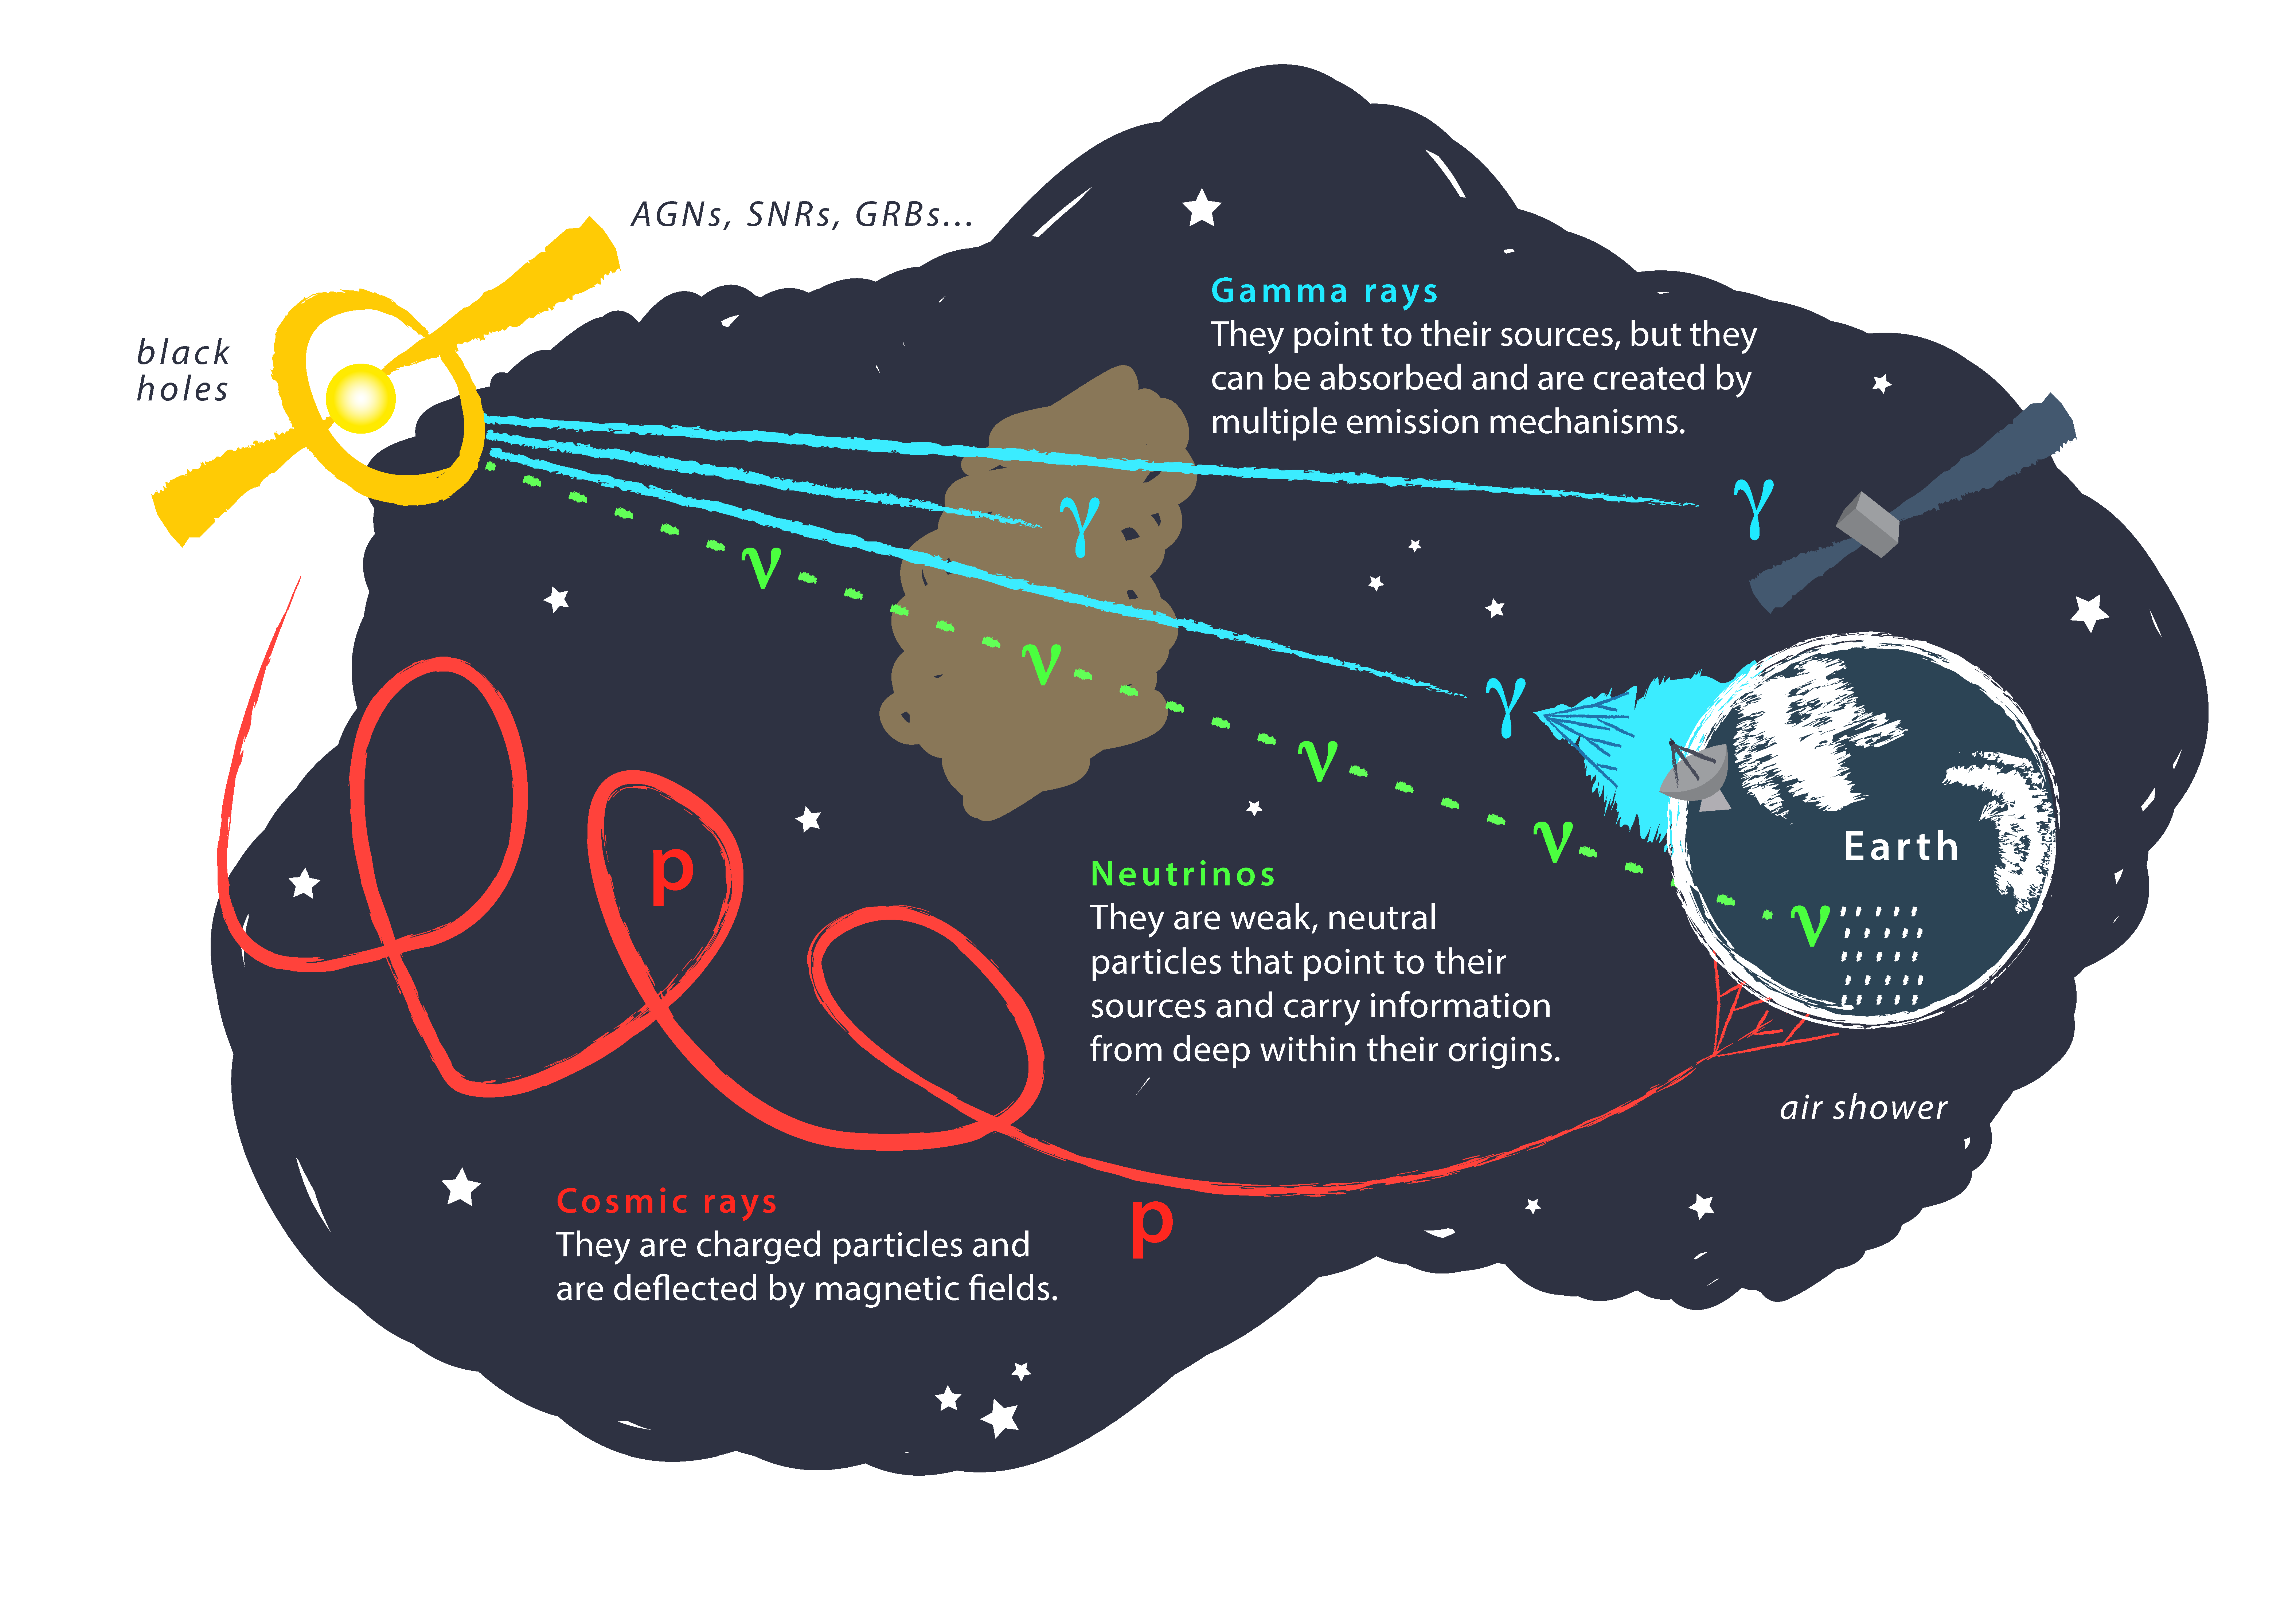
\includegraphics[width=0.9\textwidth]{images/cosmic_messengers.png}
    \caption{Only uncharged particles carry information about their origin when they arrive on earth.
        Neutrinos are hard to detect as they only interact via the weak force.
        Photons on the other hand can be absorbed in gas clouds, but are detectable using satellite- and ground-based observeratories.
    }
    \label{fig:mma}
\end{figure}

Photons and neutrions are of special interest as they are not influenced by cosmic electromagentic fields and therefore it is possible to reconstructed their origin 
position and study their sources.
As high energy gamma radiation cannot be produced thermally, more complex processes involving charged particles (Cosmic Rays) have to be considered 
(Further information in \cite{s_funk}).

The most important source class within our own galaxy are supernova remnants like the Crab Nebula \cite{nuimeprn12618}. 
Because of its constantly high gamma ray flux the Crab Nebula is often used as a "standart candle" in Gamma Ray Astronomy, observations of which are also 
analysed as part of this work.
Extragalactic sources for gamma rays are mostly supermassive black holes at the center of very bright galaxies, so called active galactic nuclei (AGN).
These black holes accrete matter from its surroundings resulting in the formation of disks around the black holes and sometimes relativistic jets are emitted 
perpendicular to the disk.
AGNs are classified depending on if a jet is emitted, how bright they are and at which angle they are observed as shown in \autoref{fig:agn}.
One of closest to earth examples of a blazar is Markarian 421 located at a redshift of $z = \num{0.03}$ \cite{Albert_2007} and observations of it are analysed in 
\autoref{ch:results}.
\begin{figure}
    \centering
    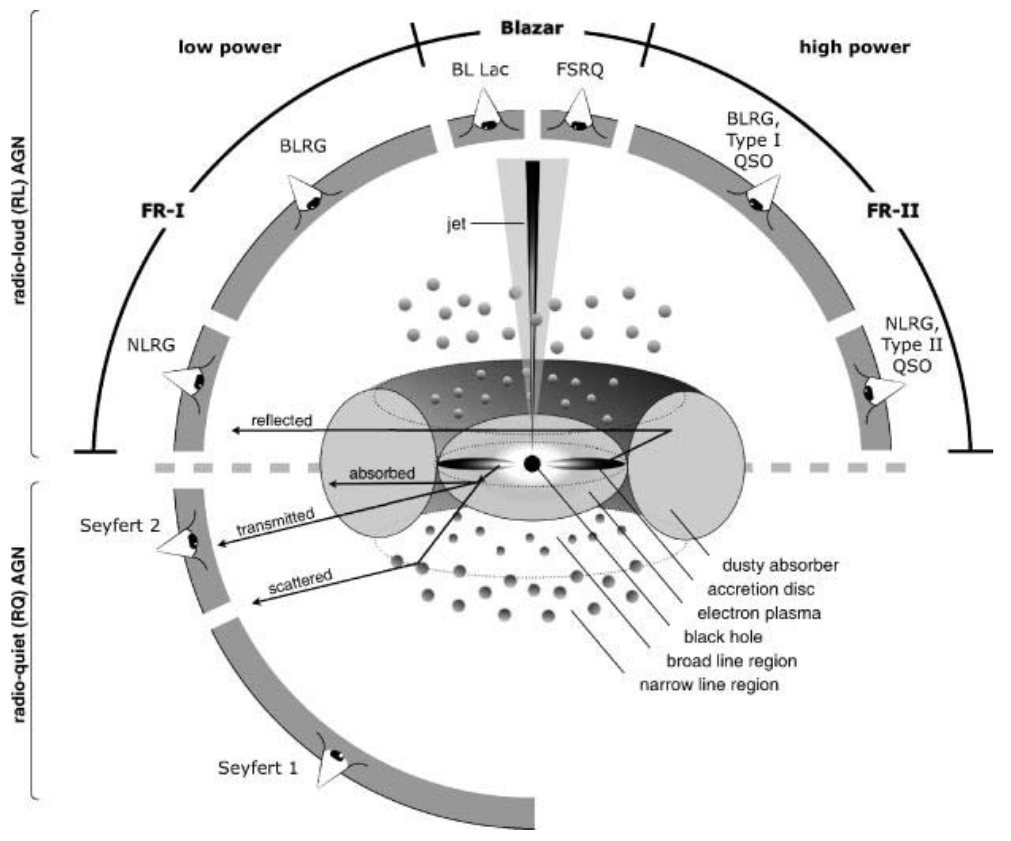
\includegraphics[width=0.8\textwidth]{images/agn.png}
    \caption{AGNs consist of a supermassive black hole in the center surrounded by an accretion disc which is again surrounded by a gas torus.
        The calssification of AGNs is based on three main characteristics, the existence of a jet, their brightness and the angle under which they can be observed \cite{doi:10.1002/9783527666829.ch4}.
    }
    \label{fig:agn}
\end{figure}


As earth's atmosphere is not transparent for high energy gamma rays, direct observations of gamma rays can only be done by satellite based observeratories 
like the Large Area Telescope on the \textit{Fermi} Gamma-Ray Space Telescope (\textit{Fermi}-LAT).
On the ground indirect observations are possible by using Imaging Air Cherenkov Telescopes (IACTs) which will be explained further in \autoref{ch:cta}.
